\documentclass[10pt,letterpaper]{article}

% --------------------------------------------------
% Packages
% --------------------------------------------------
\usepackage[utf8]{inputenc}
\usepackage[T1]{fontenc}


\usepackage{amsmath,amssymb}
\usepackage{geometry}
\usepackage{fancyhdr}
\usepackage{enumitem}
\usepackage{graphicx}
\usepackage{xcolor}
\usepackage{listings}
\usepackage{booktabs}
\usepackage{parskip}
\usepackage{microtype}
\usepackage{tcolorbox}
\tcbuselibrary{breakable}

% --- Packages ---
\geometry{margin=2.5cm}
\usepackage{array}
\usepackage{titlesec}
\usepackage{float}
\usepackage{xurl}
\usepackage[hidelinks]{hyperref}
\usepackage{mwe}
\usepackage[spanish]{babel}
\usepackage{lastpage}

% --------------------------------------------------
% Page layout
% --------------------------------------------------
\geometry{
  top=2.0cm,
  bottom=2.0cm,
  left=2.0cm,
  right=2.0cm
}

\setlength{\parindent}{0pt}
\setlength{\parskip}{5pt}

% --------------------------------------------------
% Header / footer
% --------------------------------------------------
\pagestyle{fancy}
\fancyhf{}

\fancyhead[L]{Competencia de Programación -- Estructuras de Datos}
\fancyhead[R]{2026-2S}

\fancyfoot[C]{\thepage}

% --------------------------------------------------
% Problem formatting
% --------------------------------------------------
\newcommand{\problem}[2]{
  \clearpage

  \section*{Problem #1 -- #2}

  \addcontentsline{toc}{section}{Problem #1 -- #2}
}

\newcommand{\inputsection}{
  \subsection*{Entrada}
}

\newcommand{\outputsection}{
  \subsection*{Salida}
}

\newcommand{\samples}{
  \subsection*{Sample input}
}

\newcommand{\sampleoutput}{
  \subsection*{Sample output}
}

\newcommand{\explanation}{
  \subsection*{Explicación}
}

% --------------------------------------------------
% Sample I/O
% --------------------------------------------------
\lstset{
  basicstyle=\ttfamily\small,
  columns=fullflexible,
  frame=single,
  breaklines=true,
  showstringspaces=false
}


\newenvironment{sample}[2]{
  \begin{tcolorbox}[title=Prueba \##1, colback=white, colframe=black, sharp corners,
    fonttitle=\bfseries, breakable]
    \begin{tabular}{|p{0.45\linewidth}|p{0.45\linewidth}|}
      \hline
      \textbf{Entrada} & \textbf{Salida} \\
      \hline
      }{\\ \hline
    \end{tabular}
  \end{tcolorbox}
}


% --------------------------------------------------
% Document
% --------------------------------------------------
\begin{document}

\pagenumbering{gobble}
% ==================================================
% COVER
% ==================================================

\begin{titlepage}

  \centering

  \vspace*{2cm}

  {\Large\bfseries Competencia de Programación - Estructuras de Datos\par}

  \vspace{0.5cm}

  {\Huge\bfseries 2026-2S\par}

  \vspace{1.5cm}

  {\Large Este set de problemas tiene 4 problemas, ennumerados de la página 1 a la \pageref{last-page}\par}

  \vspace{0.5cm}

  {\large \today\par}

  \vfill

  {\large
    Facultad de Ciencias Naturales e Ingeniería\\
    Universidad Jorge Tadeo Lozano
    \par}

  \vspace{1cm}

  {\large
    Todos los problemas son de autoría por Ludwig Alvarado o adaptados de \url{https://codeforces.com}
    \par}

\end{titlepage}


% ==================================================
% GENERAL INFORMATION
% ==================================================

\section*{Información General}

Salvo que se indique lo contrario, las siguientes condiciones aplican a todos los problemas.

\subsection*{Entrada}

\begin{enumerate}[leftmargin=*]
  \item La entrada se lee desde la entrada estándar.
  \item Existe múltiples casos de prueba.
  \item Los valores de una misma línea están separados por espacios.
  \item No hay datos adicionales en la entrada.
\end{enumerate}

\subsection*{Salida}

\begin{enumerate}[leftmargin=*]
  \item La salida se escribe en la salida estándar.
  \item Debe imprimirse exactamente el resultado solicitado, sin información adicional.
\end{enumerate}


\subsection*{Material y herramientas permitidas}

\begin{enumerate}[leftmargin=*]
  \item Se permite utilizar únicamente material de consulta \textbf{impreso}, como libros, apuntes y hojas de referencia.
  \item También se permite consultar exclusivamente:
        \begin{itemize}
          \item Python: \url{https://docs.python.org/}
          \item Java: \url{https://docs.oracle.com/en/java/}
          \item C/C++: \url{https://cppreference.net/}
        \end{itemize}
  \item No está permitido consultar ninguna otra página web, utilizar buscadores, foros, blogs, repositorios, sitios de soluciones ni fuentes externas.
  \item No se permite el uso de celulares, relojes inteligentes, audífonos, tabletas u otros dispositivos personales. Estos deberán permanecer \textbf{guardados en la maleta durante toda la sesión}.
  \item Está prohibido utilizar LLM, asistentes de inteligencia artificial o herramientas de generación automática de código, incluyendo ChatGPT, GitHub Copilot, Gemini, Claude o equivalentes.
  \item El único IDE permitido es \textbf{USACO Guide IDE}, disponible en \url{https://ide.usaco.guide/}. Los lenguajes permitidos son \textbf{C/C++, Java y Python}.
\end{enumerate}

\subsubsection*{Comunicación y colaboración}

\begin{enumerate}[leftmargin=*]
  \item Los integrantes del grupo pueden discutir problemas, diseñar algoritmos, revisar código y tomar decisiones conjuntamente.
  \item Está prohibido recibir o proporcionar ayuda a otros grupos, así como compartir código, algoritmos, soluciones o fragmentos de código.
  \item Las consultas al profesor se limitarán a dudas sobre la \textbf{lectura o interpretación de los datos de entrada}. No se proporcionarán pistas sobre algoritmos, estrategias, complejidad o soluciones, ni se revisarán o validarán códigos.
  \item No está permitido comunicarse con personas externas al grupo para obtener ayuda, ni observar o copiar información de otros grupos.
\end{enumerate}


% ==================================================
% PROBLEM A
% ==================================================



\problem{A}{Sandía}
{\vspace{-0.5cm} \scriptsize (Original en Codeforces: Watermelon)}

\pagenumbering{arabic}
En un caluroso día de verano, Pete y su amigo Billy decidieron comprar una sandía. En su opinión, eligieron la más grande y madura. Después de eso, pesaron la sandía y la báscula indicó que pesaba $w$ kilogramos. Regresaron corriendo a casa, muertos de sed, y decidieron dividir la sandía. Sin embargo, se enfrentaron a un problema difícil.

Pete y Billy son grandes aficionados a los números pares, por lo que quieren dividir la sandía de tal manera que cada una de las dos partes pese un número par de kilogramos. Al mismo tiempo, no es obligatorio que las partes sean iguales. Los niños están extremadamente cansados y quieren comenzar a comer lo antes posible, por lo que debes ayudarlos a determinar si pueden dividir la sandía de la manera que desean.

Por supuesto, cada uno de ellos debe recibir una parte de peso positivo.

\inputsection

La primera y única línea de entrada contiene un número entero $w$
($1 \leq w \leq 100$), que representa el peso de la sandía comprada por los niños, en kilogramos.

\outputsection

Imprime \texttt{YES} si los niños pueden dividir la sandía en dos partes, cada una con un peso par de kilogramos. En caso contrario, imprime \texttt{NO}.

\begin{sample}{1}{}
  \texttt{8}

  &

  \texttt{YES}
\end{sample}

\explanation

Por ejemplo, los niños pueden dividir la sandía en dos partes de $2$ y $6$ kilogramos, respectivamente. Otra posibilidad es dividirla en dos partes de $4$ y $4$ kilogramos.



% ==================================================
% PROBLEM B
% ==================================================

\problem{B}{Cabito Organizadito}

Cabito (figura \ref{fig:cabos} a la izquierda) es la mascota de la Universidad Jorge Tadeo Lozano. Él es el sucesor de Cabo (figura \ref{fig:cabos} a la derecha, lo vamos a llamar Don Cabo), un perrito muy querido por toda la comunidad Tadeísta (al igual que Cabito) hace muchos años\ldots Cabito llego como un compañero de Don Cabo y es el que hoy en día conocemos en la Tadeo. Estos dos amados perritos en el corto tiempo que estuvieron juntos se pasaron algunas \textit{mañas}, en especial Don Cabo (como gran mentor) a Cabito.


\begin{figure}[H]
  \centering
  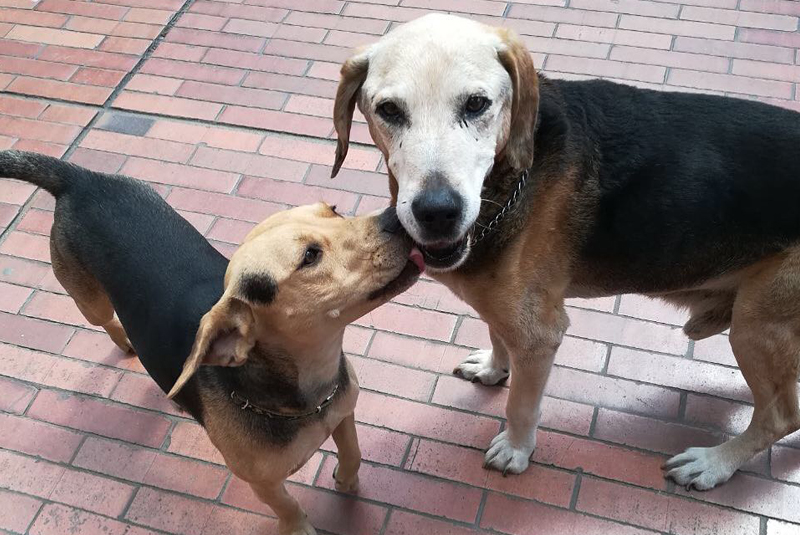
\includegraphics[width=0.6\textwidth]{img1.jpg}
  \caption{Cabito y Cabo. Autor de la foto: Universidad Jorge Tadeo Lozano}
  \label{fig:cabos}
\end{figure}


Entre una de las muchas \textit{mañas}, está la comida\ldots Don Cabo en un día de enseñanzas a Cabito le dijo: ``\textit{guau guau, guauuu guau guau woof, woof guau woooof\ldots}'' En español esto quiere decir ``Cabito, cuando tengas hambre, pídele comida a esos ingenuos estudiantes\ldots'' Siguiendo sus aprendizajes, Cabito mira con sus tiernos ojos a los estudiantes en busca de comida y ellos le dan (\textbf{¡Nunca le debes dar comida a Cabito!}).

Cada vez que alguien le da comida a Cabito él se va a su \textit{guarida secreta} y coloca la comida que le han dado en el suelo y organiza las unidades de comida por filas. Cabito sigue el siguiente patrón; en la primera fila coloca 1 unidad de comida, en la segunda fila coloca 2 unidades de comida, y así sucesivamente, entonces en la fila \(i\) Cabito coloca \(i\) unidades de comida.

Al final de cada día Cabito quiere saber cuántas filas de comida puede organizar y tu misión es escribir un programa para ayudarlo.

\inputsection

Cabito te va a dar un número entero (\(1 \leq n \leq 100\)), la cantidad total de unidades de comida que logró recolectar a lo largo del día. Recuerda que Cabito organiza su comida por filas y en la primera fila debe haber 1 unidad de comida, en la segunda fila 2 unidades de comida, en la tercera fila 3 unidades de comida y así sucesivamente\ldots

\outputsection


Lo que tu programa debe hacer es imprimir un número entero, la cantidad de filas que Cabito puede formar con el \(n\) dado. Si Cabito te da \(n = 3\) (tres unidades de comida), en la primera fila hay una unidad de comida y en la segunda dos. Por lo tanto, lo que debes imprimir es \texttt{2} (porque hay 2 filas en total). Sin embargo, hay un detalle extra, en la fila \(i\) \textbf{deben haber mínimo} \(i\) unidades de comida. Es decir, en el caso de que Cabito te de \(n=4\) la comida se debe organizar así; en la primera fila una unidad de comida, en la segunda fila \textbf{3} unidades de comida. Esto se debe a que para tener una tercera fila deben haber \textbf{mínimo} 3 unidades de comida, por lo tanto, para el caso \(n = 4\) tu programa debe imprimir \texttt{2}.


\begin{sample}{1}{}
  \texttt{3}
  &
  \texttt{2}
\end{sample}

\begin{sample}{2}{}
  \texttt{6}
  &
  \texttt{3}
\end{sample}

\begin{sample}{3}{}
  \texttt{4}
  &
  \texttt{2}
\end{sample}

\explanation

En la primera prueba, Cabito reparte \texttt{3} unidades: pone 1 en la primera fila y 2 en la segunda, usando en total \texttt{2} filas.

En la tercera prueba, con \texttt{4} unidades: coloca 1 en la primera fila y 3 en la segunda. No alcanza para una tercera (que requeriría 6 unidades en total, vea prueba 2), así que también se usan \texttt{2} filas.

% ==================================================
% PROBLEM C
% ==================================================

\problem{C}{Votación Hexagonal}

Dentro de la Universidad Tecnológica de Algoritmos y Desarrollo Optimizado (UTADEO), se están organizando las próximas elecciones para representantes estudiantiles al consejo directivo. Debido a la polémica que hubo el año pasado por un posible fraude, la universidad decidió seleccionar 6 puntos físicos vigilados para que los estudiantes puedan ir a votar que se pueden ver en la figura~\ref{fig:1}.

\begin{figure}[H]
  \centering
  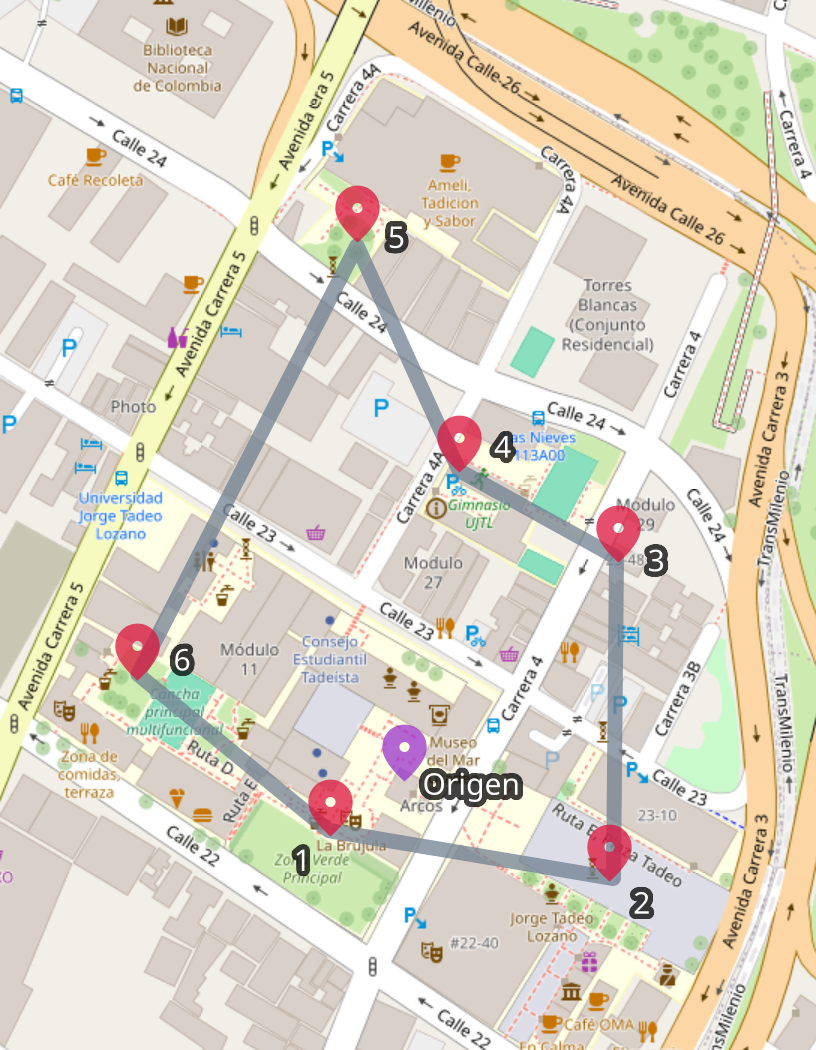
\includegraphics[width=0.4\textwidth]{img2.png}
  \caption{Puestos de votación disponibles, datos cartográficos de OpenStreetMap, edición por autoría propia.}
  \label{fig:1}
\end{figure}


Debido a que este año la universidad asignó un presupuesto mucho mayor, te contrataron a ti como programador para mostrar los resultados de las elecciones, distancia del puesto de votación más lejano al origen, y el Índice Energético de Votación (IEV) definido como:

\[
  IEV = \lceil \sqrt[3]{V} \rceil !
\]

Donde \(V\) es la cantidad de votos totales en una mesa de votación. Para este año se postularon 3 estudiantes para ser el nuevo representante al consejo directivo de la universidad, ellos son; Andrea (\(A\)), Bobby (\(B\)) y Claudia (\(C\)).

\inputsection

Vas a recibir 6 líneas de datos, en cada línea vas a encontrar las coordenadas \((x, y), \ (-1000 < x, y < 1000)\) de cada puesto de votación con respecto al origen \((0, 0)\) seguido de la cantidad de votos que tuvo Andrea, Bobby y Claudia en esa mesa de votación, (\(1 \leq A, B, C \leq 500\)).

\outputsection

Se deben imprimir el total de votos de todas las mesas de votación, la cantidad de votos que tuvo cada candidato en todas las mesas, el porcentaje de votos de cada candidado, la mesa más lejana al origen y el IEV del puesto de votación con más votos recogidos.

Se debe seguir el siguiente formato:


\noindent\texttt{Total Votos: \#numeroVotos\\Votos Andrea: \#votos \#porcentaje\\Votos Bobby: \#votos \#porcentaje\\Votos Claudia: \#votos \#porcentaje\\Mesa más lejana: \#numeroMesa \#distancia\\IEV: \#numeroMesa \#valorIEV}

\begin{sample}{1}{}
  \texttt{-1 -1 78 50 90}

  \texttt{5 -1 100 90 115}

  \texttt{3 7 20 15 10}

  \texttt{0 8 40 55 30}

  \texttt{-2 11 470 450 370}

  \texttt{-7 2 90 95 80}

  &

  \texttt{Total Votos: 2248}

  \texttt{Votos Andrea: 798 35.50}

  \texttt{Votos Bobby: 755 33.59}

  \texttt{Votos Claudia: 695 30.92}

  \texttt{Mesa mas lejana: 5 11.18}

  \texttt{IEV: 5 39916800}
\end{sample}


% ==================================================
% PROBLEM D
% ==================================================

\problem{D}{Los números de Cabito}

En la Universidad Tecnológica de Algoritmos y Desarrollo Optimizado (UTADEO), Cabito ha decidido que quiere aprender programación para poder ayudar a los estudiantes en sus clases. Como todavía está aprendiendo, su profesor decidió comenzar con un ejercicio sencillo sobre números pares e impares.

Un día, Cabito encontró una lista de números que algunos estudiantes habían dejado en un computador de la universidad. Como Cabito es un perrito muy organizado, decidió revisar cada uno de los números de la lista y clasificarlos.

Sin embargo, Cabito todavía no sabe contar muy bien. Por eso, necesita tu ayuda para determinar cuántos números pares y cuántos números impares hay en la lista.

\inputsection

La primera línea contiene un entero $N$ ($1 \leq N \leq 1000$), que representa la cantidad de números que hay en la lista.

La segunda línea contiene $N$ números enteros $a_1,a_2,\ldots,a_N$ ($-10^9 \leq a_i \leq 10^9$).

\outputsection

Debes imprimir dos números enteros: primero, la cantidad de números pares de la lista, y segundo, la cantidad de números impares.

Los dos números deben estar separados por un espacio.

\begin{sample}{1}{}
  \texttt{5}

  \texttt{1 2 3 4 5}

  &

  \texttt{2 3}
\end{sample}

\begin{sample}{2}{}
  \texttt{8}

  \texttt{10 7 4 9 12 15 20 21}

  &

  \texttt{4 4}
\end{sample}

\begin{sample}{3}{}
  \texttt{6}

  \texttt{-2 -5 0 8 11 13}

  &

  \texttt{3 3}
\end{sample}

\explanation

En la primera prueba, la lista contiene los números $1,2,3,4,5$. Los números pares son $2$ y $4$, por lo que hay \texttt{2} números pares. Los números impares son $1$, $3$ y $5$, por lo que hay \texttt{3} números impares.

En la segunda prueba hay cuatro números pares: $10$, $4$, $12$ y $20$. Los cuatro números restantes son impares.

En la tercera prueba, los números pares son $-2$, $0$ y $8$, mientras que $-5$, $11$ y $13$ son impares. Por lo tanto, la respuesta es \texttt{3 3}.


\label{last-page}


\end{document}
